\section{Introduction}
There is a growing increasing interest in \emph{spatial processor} architectures with a physically distributed control unit (for e.g. Program Memory), because they provide a feasible solution to enable both energy savings and performance gains over processors with cetralized control unit~\cite{7284058,8686088}. %thus matching current application demands.
%ADDCITATION ((2013). The End of Dennard Scaling. Accessed: Feb. 2013. [Online].
%Available: https://cartesianproduct.wordpress.com/2013/04/15/the-endof-dennard-scaling/
%[3] H. Esmaeilzadeh, E. Blem, R. S. Amant, K. Sankaralingam, and
%D. Burger, “Dark silicon and the end of multicore scaling,” in Proc.
%38th Annu. Int. Symp. Comput. Archit. (ISCA), Jun. 2011, pp. 365–376.}
Despite the growing interest, the design of spatial processors remains challenging due to the lack of automated tools. Moreover, since there is compelling evidence that the memory system (both on-chip and off-chip) has become a dominant factor affecting the overall performance~\cite{williams2009roofline}, power consumption~\cite{dayarathna2015data}, and silicon area usage~\cite{oh2009analytical}, new design methods \textit{must} take the memory-system into account while designing spatial processors.
In fact, given that the memory system and the processing elements in a spatial processor architecture are so tightly \textit{interdependent}, we argue they must be \textit{co-designed}. This is especially important while considering using emerging memory technologies, such as MRAM, eDRAM, PCM, or RRAM~\cite{mem2016} in spatial processors: they have higher integration density and lower power than SRAM, but also come with additional "quirks" (e.g., MRAM features different read and write latencies).

%
%BibTeX | EndNote | ACM Ref
%@inproceedings{Hameed:2010:USI:1815961.1815968,
% author = {Hameed, Rehan and Qadeer, Wajahat and Wachs, Megan and Azizi, Omid and Solomatnikov, Alex and Lee, Benjamin C. and Richardson, Stephen and Kozyrakis, Christos and Horowitz, Mark},
% title = {Understanding Sources of Inefficiency in General-purpose Chips},
% booktitle = {Proceedings of the 37th Annual International Symposium on Computer Architecture},
% series = {ISCA '10},
% year = {2010},
% isbn = {978-1-4503-0053-7},
% location = {Saint-Malo, France},
% pages = {37--47},
% numpages = {11},
% url = {http://doi.acm.org/10.1145/1815961.1815968},
% doi = {10.1145/1815961.1815968},
% acmid = {1815968},
% publisher = {ACM},
% address = {New York, NY, USA},
% keywords = {ASIC, chip multiprocessor, customization, energy efficiency, h.264, high performance, tensilica},
%}

Many CAD tools~\cite{synopsystool,tensilica,codasiptool} help alleviate the increasing design complexity of typical custom-processor in which there is a single Program/Instruction memory. However, selecting an optimal spatial processor architecture, taking into account the various trade-offs in latency, power consumption, and area usage still requires extensive design-space exploration (DSE) and cannot be performed using the existing CAD tools.
In addition, state-of-the-art design flows for custom-processor design-space exploration focus on processor architecture optimization~\cite{Meloni2012,EusseSAMOS2014,Jozwiak2013,Karuri2009}, and do not include the memory system, as illustrated in Figure~\ref{fig:intro}. Co-optimization of the processor and the memory system (including emerging memories) is typically done by co-simulation, and/or by optimizing the cache replacement policy~\cite{4798259,7092595,6271803,Mittal13f}.
%Papers to cite for CDFG generation and Application Specific High LSynthesis~\cite{Coussy:2008:HSA:1457713,Kato2008}.
On the other hand, emerging spatial architectures~\cite{7284058,8686088}, which distribute the program memory and processing elements to achieve maximum performance use rigid interconnect topologies to allow flexible communication between processing elements leading to larger area and power utilization.

\begin{figure}[ht]
    \centering
    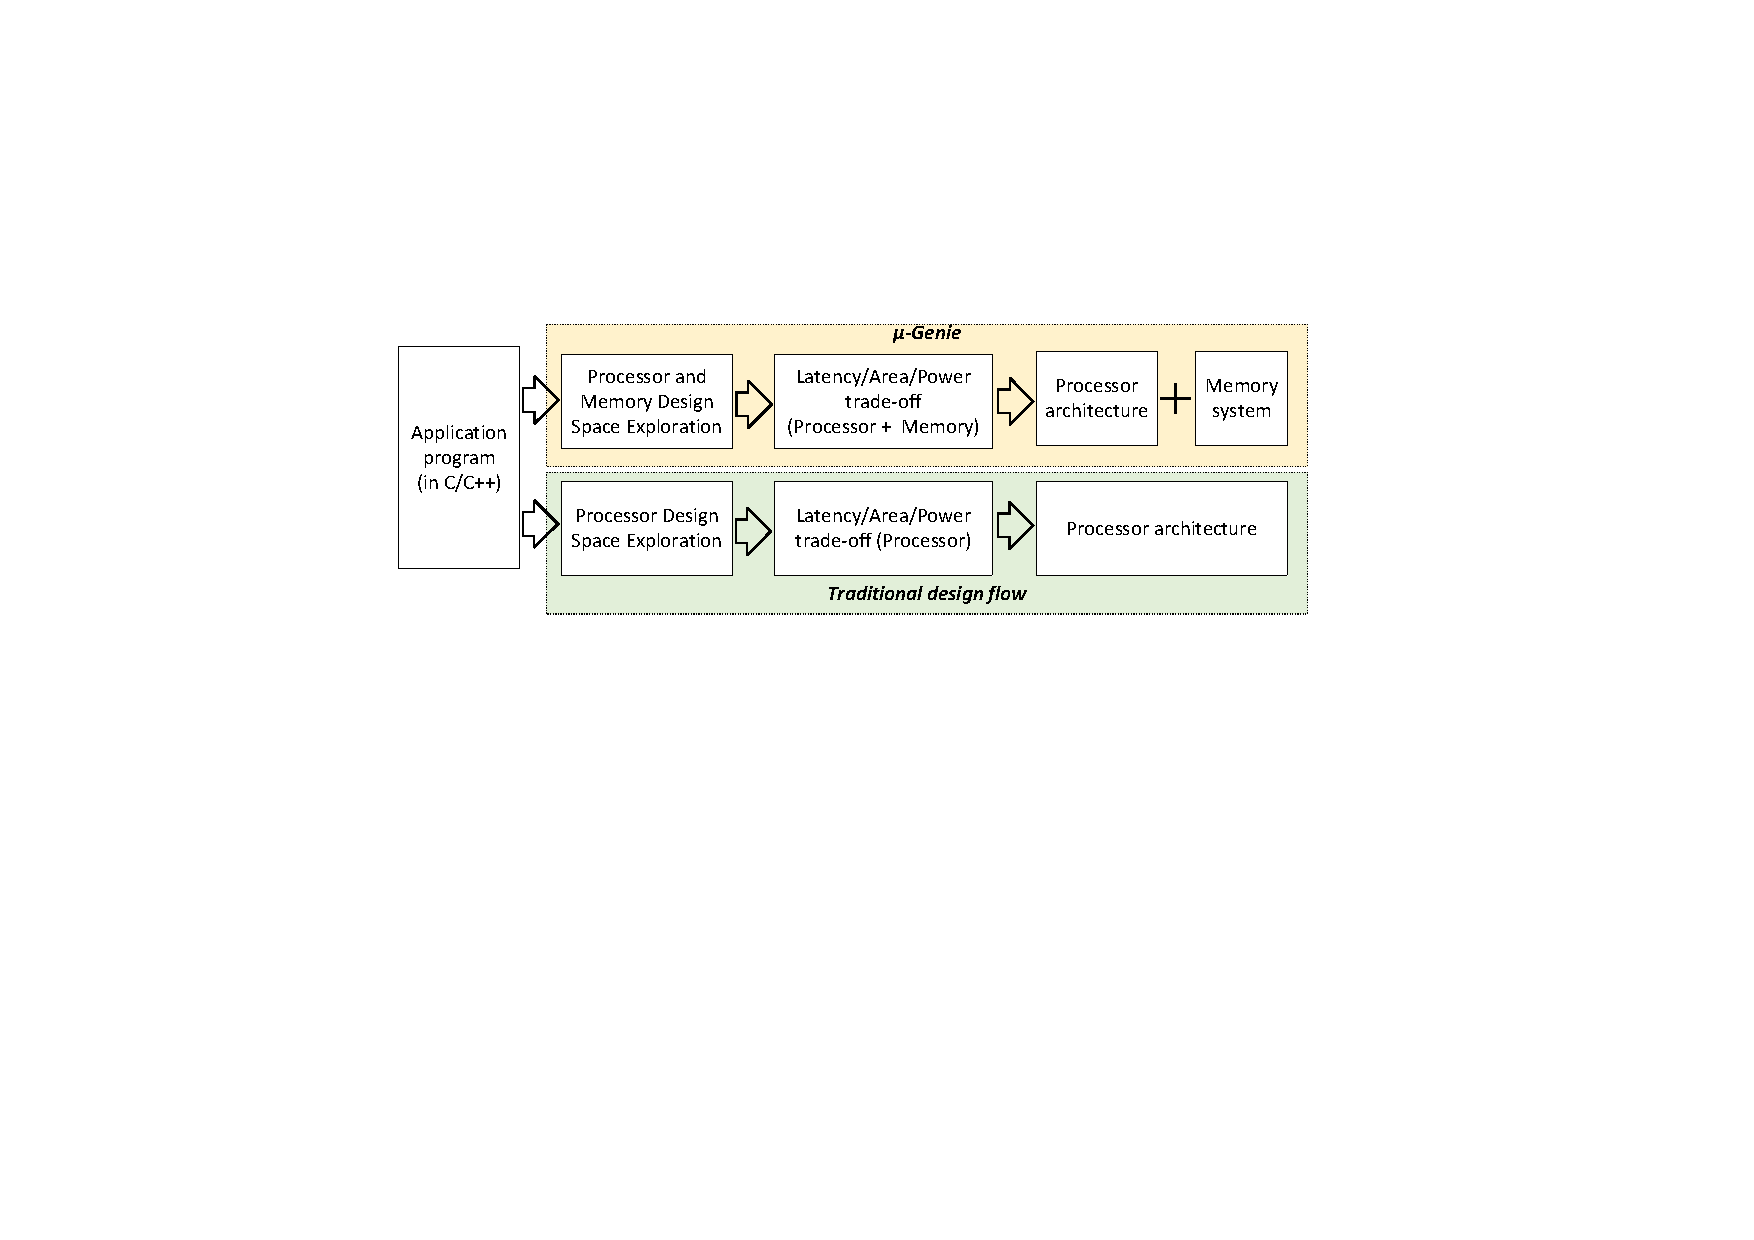
\includegraphics[clip, trim=6cm 10.5cm 6.4cm 5.2cm, width=1.0\linewidth]{images/intro_figure.pdf} %[left down right up ]
    \caption{\small Difference between state-of-the-art design flow typically used for non-spatial processor architecture and the proposed \frameworkname~design flow for spatial processor architecture design.}
    \label{fig:intro}
\end{figure}

In this work, we propose \frameworkname (\ref{sec:framework}), a novel automated framework for \textit{memory-aware spatial processor design-space exploration}, which enables users to explore various architectural trade-offs for the joined (processor, memory system) ensemble. The framework allows unprecedented configuration options: memory levels technologies (novel among similar tools), clock frequency (per memory level, also novel), read/write latency (potentially different), and data width. Thus, our \frameworkname~is the first to enable design-space exploration for application-specific spatial processors beyond state-of-the-art solutions, even enabling a first comparison between different memory technologies, like MRAM and SRAM (Section~\ref{sec:case_studies}).

Moreover, \frameworkname~uses spatial architectural templates (Section~\ref{sec:arch_template}) to actually generate ready-to-use spatial processor designs. These designs can be configured at design-time (based on the trade-off from the framework), and allow for fast prototyping of application-specific hardware.

To demonstrate the capabilities of \frameworkname, we cover three case-studies, showing how spatial processor can be designed for two different applications and many configurations, even those using MRAM or SRAM for the memory system, can be generated, analysed, and compared (Section~\ref{sec:case_studies}).



 %Ana: if you keep this format, without the contributions specifically listed, this final paragraph (below) is not well-positioned. You might want ti add this at the beginning of "In this work..." paragraph - I added it there for you to see what I mean. This summary is only needed here if you go for the bullet-point-like contributions.
 %\frameworkname~enables design space exploration for application-specific custom-processors beyond the current state-of-the-art solutions, even enabling a first comparison between different memory technologies, like MRAM and SRAM.

%In this work we present \frameworkname, a framework that allows to compare design choices and perform automatic system level design and implementation. We propose a novel memory-driven approach for application-specific hardware design starting from two observations. First, the memory system and the processing system are \textit{interdependent} and therefore they should be \textit{co-designed}. Second, the \textit{data dependencies} of the fixed application impose constaints on the design of both memory and processing systems. Hence, our approach starts from the analysis of an input application and codesigns memory and custom processor, shown in Figure~\ref{fig:intro}.
